\documentclass[usenames,dvipsnames]{beamer}

\mode<presentation> {

% The Beamer class comes with a number of default slide themes
% which change the colors and layouts of slides. Below this is a list
% of all the themes, uncomment each in turn to see what they look like.

%\usetheme{default}
%\usetheme{AnnArbor}
%\usetheme{Antibes}
%\usetheme{Bergen}
%\usetheme{Berkeley}
%\usetheme{Berlin}
%\usetheme{Boadilla}
\usetheme{CambridgeUS}
%\usetheme{Copenhagen}
%\usetheme{Darmstadt}
%\usetheme{Dresden}
%\usetheme{Frankfurt}
%\usetheme{Goettingen}
%\usetheme{Hannover}
%\usetheme{Ilmenau}
%\usetheme{JuanLesPins}
%\usetheme{Luebeck}
%\usetheme{Madrid}
%\usetheme{Malmoe}
%\usetheme{Marburg}
%\usetheme{Montpellier}
%\usetheme{PaloAlto}
%\usetheme{Pittsburgh}
%\usetheme{Rochester}
%\usetheme{Singapore}
%\usetheme{Szeged}
%\usetheme{Warsaw}

% As well as themes, the Beamer class has a number of color themes
% for any slide theme. Uncomment each of these in turn to see how it
% changes the colors of your current slide theme.

%Custom color scheme 
    % https://cals.cornell.edu/faculty-staff/marketing-communications/resources/brand-guide/visual-identity/color-typography
    % Primary Palette
    \definecolor{Cornellian}{RGB}{179,27,27}
    \definecolor{PMSCoolGray11}{RGB}{85,86,90}
    \definecolor{PMS430C}{RGB}{125,134,140}
    \definecolor{PMSCoolGray4C}{RGB}{189,187,187}
    \definecolor{PMSCoolGray1C}{RGB}{242,242,242}
    \definecolor{White}{RGB}{255,255,255}
    % Secondary Palette
    \definecolor{PMSRed032}{RGB}{239,64,53}
    \definecolor{PMS7462}{RGB}{0,104,172}
    \definecolor{PMSProcessBlue}{RGB}{55,135,176}
    \definecolor{PMS7458}{RGB}{137,204,226}
    \definecolor{PMS369}{RGB}{110,180,63}
    \definecolor{PMS7493}{RGB}{201,214,165}
    \definecolor{PMS5635}{RGB}{159,173,159}
    \definecolor{PMS403}{RGB}{162,153,139}

% Now set the colors you want
    
    \setbeamercolor*{palette primary}{bg=Cornellian, fg = White}
    \setbeamercolor*{palette secondary}{bg=PMSCoolGray4C, fg = Cornellian}
    \setbeamercolor*{palette tertiary}{bg=PMSCoolGray1C, fg = Cornellian}
    
    \setbeamercolor*{author in head/foot}{parent=palette primary}
    \setbeamercolor*{title in head/foot}{parent=palette tertiary}
    \setbeamercolor*{date in head/foot}{parent=palette secondary}

    \setbeamercolor*{section in head/foot}{parent=palette primary}
    \setbeamercolor*{subsection in head/foot}{parent=palette secondary}
    
    \setbeamercolor*{external link}{parent=palette secondary}
    
    \setbeamercolor*{titlelike}{bg = PMS430C, fg = Cornellian}
    \setbeamercolor*{title}{bg=Cornellian, fg = White}
    \setbeamercolor*{item}{fg=PMS7462}
    \setbeamercolor*{caption name}{fg= White}
    \setbeamercolor*{button}{bg=Cornellian,fg=white}

%\setbeamercolor{button}{bg=Maroon,fg=white}
%\setbeamercolor{block title}{bg=Maroon,fg=white}
%\setbeamertemplate{footline} % To remove the footer line in all slides uncomment this line
%\setbeamertemplate{footline}[page number] % To replace the footer line in all slides with a simple slide count uncomment this line

%\setbeamertemplate{navigation symbols}{} % To remove the navigation symbols from the bottom of all slides uncomment this line
}

\usepackage{graphicx} % Allows including images
\usepackage{booktabs} % Allows the use of \toprule, \midrule and \bottomrule in tables
\usepackage{amssymb}
\usepackage{caption}
\usepackage{amsmath}
\usepackage{units}
\usepackage{pgfplots}
\usepackage{forest}
\usepackage[]{titlepic}
\usepackage{adjustbox}
\usepackage{appendixnumberbeamer}
\usepackage{bm}
\usepackage[authoryear]{natbib}
\usepackage[compatibility=false]{caption}
\captionsetup{labelformat=empty,labelsep=none}
\usepackage{amsbsy}
\usepackage[dvipsnames]{xcolor}
\usepackage{bbm}
\pgfplotsset{compat=1.12}
\usepackage{qtree}
\usepackage{tikz-qtree}
\usepackage{mathrsfs}
\usepackage{comment}
\usepackage{multirow}
\usepackage{colortbl}


%----------------------------------------------------------------------------------------
%	TITLE PAGE
%----------------------------------------------------------------------------------------

\title[Short title for footer]{Main title}

\author[Author cite in footer]{
            Author 1 \inst{1}
            \and Author 2 \inst{1}
            %\and   \inst{1} %\\ Uncomment the \\ if you need a line break
            %\and  \inst{2}
            %\and  \inst{2}
            }

\institute[]{
            \inst{1}%
            Dyson School of Applied Economics and Management | Cornell University   %\and
            %\inst{2}%
            %\and
            %\and
            } 

\date{Date}

\titlegraphic{
                % Uncomment the below and it can help push the logos down
                %\vfill
                
                % Uncomment the below and you can add a disclaimer statement.
                %\centering
                %\textit{\scriptsize Preliminary, please do not cite without permission.}
                
                \begin{columns}
                    \begin{column}{0.9\textwidth}\centering \hrule
                    \end{column}
                \end{columns} 
                \begin{columns}
                    \begin{column}{0.05\textwidth}
                    \end{column}
                    \begin{column}{0.45\textwidth} \raggedright
                        
\includegraphics[height=22pt]{Logos/Horizontal Wordmark_color.png}
                    \end{column}
                    \begin{column}{0.45\textwidth}\raggedleft
                        
\includegraphics[height=22pt]{Logos/Dyson-logo-rgb.png}
                    \end{column}
                    \begin{column}{0.05\textwidth}
                    \end{column}
                \end{columns}
                }
                
\begin{document}

%-----------------%
%	TITLE SLIDE   %
%-----------------%

\begin{frame}
    \titlepage % Print the title page as the first slide
\end{frame}

%-------------------------------%
%-------------------------------%
%      PRESENTATION SLIDES      %
%-------------------------------%
%-------------------------------%

%--------------------%
%   USDA Statement   %
%--------------------%

\begin{frame}{}
    \centering The findings and conclusions in this presentation are those of the authors and should not be construed to represent any official USDA or U.S. Government determination or policy.\\
    \vspace{10pt}
    \begin{columns}
       \begin{column}{0.5\textwidth}
    \centering   Funding provided by a cooperative agreement with:
       \end{column} 
       \begin{column}{0.5\textwidth}
    \begin{figure}
        \raggedright
        
\includegraphics[width=0.7\linewidth]{Images/usda-logo-color.png}
    \end{figure}       
    \end{column} 
    \end{columns}
\end{frame}

%-------------%
%   Roadmap   %
%-------------%

\begin{frame}{Roadmap}
    \tableofcontents
\end{frame}

%-------------------------------%
%   Background and Motivation   %
%-------------------------------%
\section{Background \& Motivation}

\begin{frame}{Background Study}
    \begin{columns}
       \begin{column}{0.5\textwidth}\centering
            Overall study objectives:
            \begin{enumerate}\tiny
                \item This is where you can discuss the background of a motivating study;
                \item There were goals;
                \item Interesting questions;
                \item Unique data.
            \end{enumerate}
       \end{column} 
       \begin{column}{0.5\textwidth}
            \begin{figure}
                \raggedright
                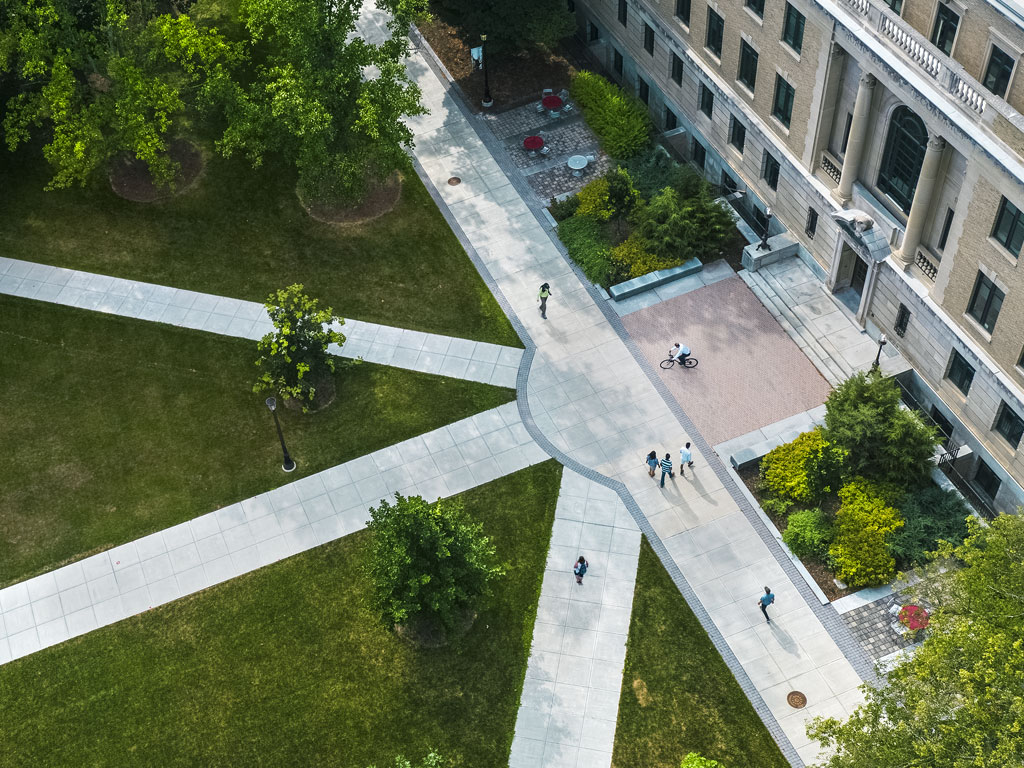
\includegraphics[width=.9\linewidth]{Images/carousel-01.jpg}
            \end{figure}       
        \end{column} 
    \end{columns}
\end{frame}

\begin{frame}{Multiple Content Slide 1}{This is a slide subtitle}
    \begin{columns}
        \begin{column}{0.35\textwidth}
            \begin{figure}
                \centering
                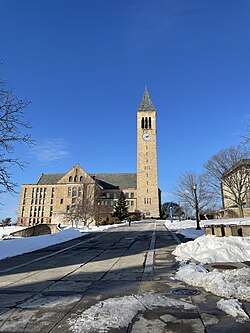
\includegraphics[width=\linewidth]{Images/McGraw_Tower_in_January.JPG}
            \end{figure} 
        \end{column} 
        \begin{column}{0.65\textwidth} \scriptsize 
            \begin{figure}
                \centering
                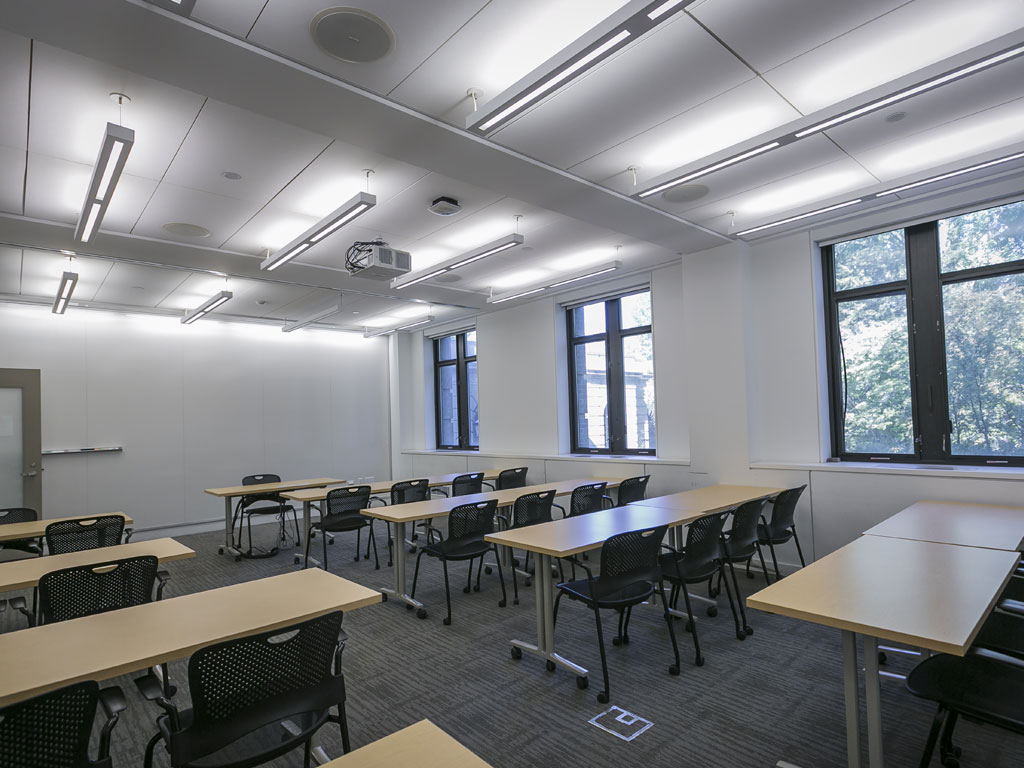
\includegraphics[width=.57\linewidth]{Images/carousel-04.jpg}
            \end{figure}
            Talk about the graphics or something else. Maybe you really like classrooms in Warren Hall and want to share them with the world \citep{Warren_food_1921}\\
            \vspace{10pt}
            \citet{Berry_food_2018} says that no previous research looks at these wonderful classrooms or the magnificent clock tower but we should!
        \end{column} 
    \end{columns}
\end{frame}

%-----------------------%
%   Research Question   %
%-----------------------%
\section{}

\begin{frame}{Research Question}
    \begin{columns}
        \begin{column}{.7\textwidth}\centering
            What is your research question? Do you need to change the width to make it look good? Did you know that you can also use \\ to manually break the lines?
        \end{column}
    \end{columns}
\end{frame}

%----------------------%
%   Data and Methods   %
%----------------------%
\section{Data \& Methods}

\begin{frame}{Data}
    \begin{itemize}
        \item This is the first data source;
        \item Another source is here;
        \item There is yet another data source to talk about;
        \item This is a dataset (and it needs clarification).
    \end{itemize}
\end{frame}

\begin{frame}{List content slide 1}
    \begin{itemize}
        \item This is a main content point;
        \begin{itemize}
            \item and there are multiple subpoints;
            \item yet another subpoint;
            \item and the final subpoint;
        \end{itemize}
        \item Another main content point;
        \item The final content point. 
    \end{itemize}
\end{frame}

%-----------------%
\subsection{Models}
%-----------------%

\begin{frame}{Example Model, Unnumbered} % The itemizes allow for the variables to not be pushed off the slide
    \begin{align*} %Use align and the & symbol to pick how equations align
        \Pr(\text{Y}_{i} = 1) &= \Phi(Z_i) \\
        Z_i &=\beta_0 + \sum_{j=1}^J\left(\alpha_j\cdot\text{A}_{ij} + \gamma_j\cdot\text{B}_{ij} \right)+\delta_{i}\cdot\text{C}_{i}+\epsilon_{i}
    \end{align*}
    \begin{itemize}
        \begin{itemize}
            \item [$i$] indexes something
            \item [$j$] indexes something else
        \end{itemize}
        \begin{itemize}
            \item [$Y_i$] Dependent variable
            \item [$\Phi(Z_i)$] Probit link (standard normal CDF)
            \item [$\text{A}_{ij}$] An independent variable
            \item [$\text{B}_{ij}$] Another independent variable
            \item [$\text{C}_{i}$] A vector of controls
            \item [$\epsilon_{i}$] Unexplained variation
        \end{itemize}
    \end{itemize}
\end{frame}

\begin{frame}{Example Model, Numbered}
    \begin{align} %Use align and the & symbol to pick how equations align
        \Pr(\text{Y}_{i} = 1) &= \Phi(Z_i) \\
        Z_i &=\beta_0 + \sum_{j=1}^J\left(\alpha_j\cdot\text{A}_{ij} + \gamma_j\cdot\text{B}_{ij} \right)+\delta_{i}\cdot\text{C}_{i}+\epsilon_{i}
    \end{align}
    \begin{itemize}
        \begin{itemize}
            \item [$i$] indexes something
            \item [$j$] indexes something else
        \end{itemize}
        \begin{itemize}
            \item [$Y_i$] Dependent variable
            \item [$\Phi(Z_i)$] Probit link (standard normal CDF)
            \item [$\text{A}_{ij}$] An independent variable
            \item [$\text{B}_{ij}$] Another independent variable
            \item [$\text{C}_{i}$] A vector of controls
            \item [$\epsilon_{i}$] Unexplained variation
        \end{itemize}
    \end{itemize}
\end{frame}

%-----------%
\subsection{}
%-----------%

\begin{frame}{Spaced list with 10pt spaces}
    \begin{itemize}
        \item This is a list that is spaced out;
        \vspace{10pt}
        \item Spacing out a list can be visually pleasant;
        \vspace{10pt}
        \item The final point.
    \end{itemize}  
\end{frame}

%-------------%
%   Results   %
%-------------%
\section{Results}

\begin{frame}{This is a basic table slide}
    \centering
    \begin{table}
    \centering
    \begin{tabular}{lccc}
        & (1) & (2) & (3) \\ \cline{2-4} 
        Avocado & 1 & 2 &  3\\
        Blueberry & 4 & 5 & 6 \\
        Cranberry & 7 & 8 & 9 \\
        Dill & 10 &  &  \\
        Edamame &  & 11 &  \\
        Fennel &  & 12 & 13 \\
        Garlic & No & Yes & No \\ \hline
        nobs & 363 & 363 & 363 \\
        RMSE & .45 & .23 & .37
    \end{tabular}
    \caption{Table captions can be moved by placing below or above tabular}
    \end{table}  
\end{frame}

\begin{frame}
    \centering
    \footnotesize{ There is no title here because the table is "large" so this is a footnote size comment instead.}
    \begin{table}
        \centering
        \resizebox{.95\textheight}{!}{\begin{tabular}{lccccccc}
            & (1) & (2) & (3) & (4) & (5) & (6) & (7) \\ 
            Apples & -0.022 &  & -0.003 &  &  &  &  \\
            & (0.031) &  & (0.046) &  &  &  &  \\
            Bananas &  & 0.006 & 0.007 &  &  &  &  \\
            &  & (0.035) & (0.051) &  &  &  &  \\
            Carrots &  &  &  & 0.101 &  &  &  \\
            &  &  &  & (0.091) &  &  &  \\
            Dates &  &  &  & -0.150 &  &  &  \\
            &  &  &  & (0.135) &  &  &  \\
            Eggplants &  &  &  & -0.065 &  &  &  \\
            &  &  &  & (0.123) &  &  &  \\
            Fiddleheads &  &  &  & 0.105 &  &  &  \\
            &  &  &  & (0.226) &  &  &  \\
            Green Beans &  &  &  & 0.054 & 0.054 & 0.050 &  \\
            &  &  &  & (0.107) & (0.095) & (0.120) &  \\
            Honeydew &  &  &  & -0.058 & -0.058 & -0.054 &  \\
            &  &  &  & (0.114) & (0.098) & (0.122) &  \\
            Iceberg Lettuce &  &  &  & -0.047 & -0.047 &  & -0.046 \\
            &  &  &  & (0.059) & (0.058) &  & (0.050) \\
            Jalapenos &  &  &  & 0.099 & 0.089 &  & 0.086 \\
            &  &  &  & (0.173) & (0.164) &  & (0.225) \\
            RMSE & 0.35 & 0.36 & 0.41 & 0.41 & 0.41 & 0.41 & 0.41 \\
            Controls & Yes & Yes & Yes & Yes & Yes & Yes & Yes \\
            nobs & 1,434 & 1,434 & 1,434 & 1,434 & 1,434 & 1,434 & 1,434 \\
        \end{tabular}} 
    \end{table} 
\end{frame}

\begin{frame}{Key Takeaways}
    \begin{itemize}
        \item Fruits and vegetables are pretty neat;\\
        \begin{itemize}
            \item Apples $\Rightarrow$ less likely to be something;
            \item Bananas $\Rightarrow$ more likely to be something;
            \item None have statistically significant marginal effects;
        \end{itemize}
        \item This is weird data that shouldn't be used for this purpose.\\
    \end{itemize}
\end{frame}

\begin{frame}{Next Steps}
    \begin{itemize}
        \item Utilize proper and related variables of interest (not fruit and vegetables when we should be measuring clock towers and classrooms);
        \item Add inline math such as $\text{ClockTower}_{\text{height}}\times 500$;
        \item Cite some sources.
    \end{itemize}
    \hyperlink{references}{\beamerskipbutton{References}}
\end{frame}

%---------%
%   Q&A   %
%---------%
\section{Q\&A}

\begin{frame}
    \centering
    \vspace{40pt}
    \huge Thank you! Questions?
    \vspace{20pt}
    \begin{columns}
        \begin{column}{.6\textwidth}
            \normalsize
            \begin{itemize}
                \item[]Corresponding Author
                \item[]Title
                \item[]Dyson School of Applied Economics and Management
                \item[]\#\#\# Warren Hall | Ithaca, NY
                \item[]email
            \end{itemize}
        \end{column}
        \begin{column}{.4\textwidth}
            \begin{figure}
                \raggedright
                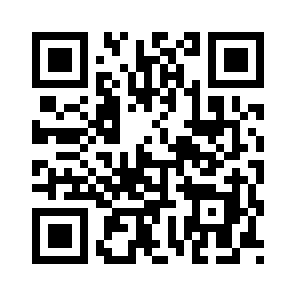
\includegraphics[width=0.7\linewidth]{Images/QR_code_for_mobile_English_Wikipedia.png}
            \end{figure}
        \end{column}
    \end{columns}
    \vspace{20pt}
    \begin{columns}
        \begin{column}{0.9\textwidth}\centering \hrule
        \end{column}
    \end{columns} \vspace{-12pt}
    \begin{columns}
        \begin{column}{0.05\textwidth}
        \end{column}
        \begin{column}{0.45\textwidth} \raggedright
            
\includegraphics[height=22pt]{Logos/Horizontal Wordmark_color.png}
        \end{column}
        \begin{column}{0.45\textwidth}\raggedleft
            
\includegraphics[height=22pt]{Logos/Dyson-logo-rgb.png}
        \end{column}
        \begin{column}{0.05\textwidth}
        \end{column}
    \end{columns}
\end{frame}

%----------------%
%   References   %
%----------------%
\section*{References}

\footnotesize
\begin{frame}[allowframebreaks]
        \frametitle{References}\label{references}
%        \nocite{*}
        \bibliographystyle{apalike}
        \bibliography{references}
\end{frame}

%--------------%
%   Appendix   %
%--------------%
\section{Appendix}

\begin{frame}{Multiple Content Slide 2}
    \begin{columns}
        \begin{column}{0.3\textwidth}
            \begin{figure}
                \raggedright
                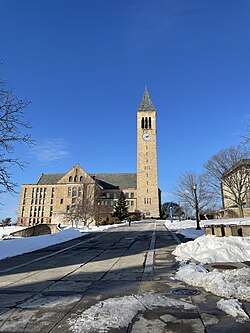
\includegraphics[width=\linewidth]{Images/McGraw_Tower_in_January.JPG}
            \end{figure} 
       \end{column} 
       \begin{column}{0.3\textwidth}
            \begin{figure}
                \raggedright
                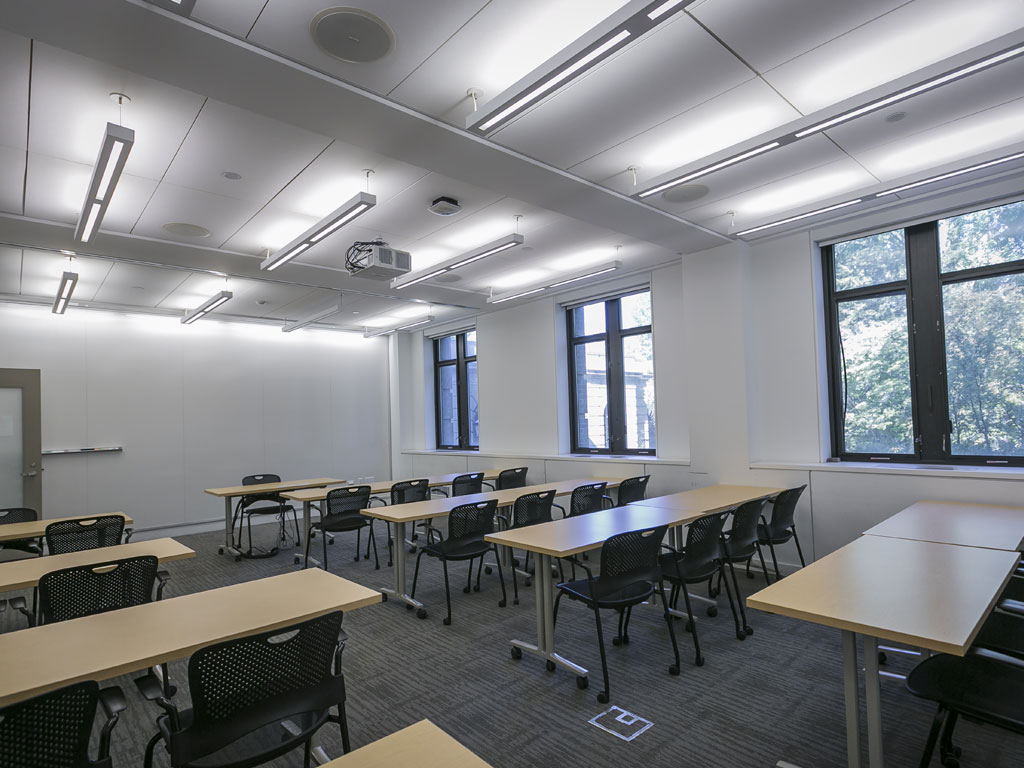
\includegraphics[width=\linewidth]{Images/carousel-04.jpg}
            \end{figure}       
        \end{column} 
    \end{columns}
    \begin{columns}
        \begin{column}{\textwidth}
            \footnotesize
             Talk about the graphics or something else. Maybe you really like classrooms in Warren Hall and want to share them with the world \citep{Warren_food_1921}\\
            \vspace{10pt}
            \citet{Berry_food_2018} says that no previous research looks at these wonderful classrooms or the magnificent clock tower but we should!
        \end{column}
    \end{columns}
\end{frame}

\end{document}